\documentclass[UTF8]{ctexart}
%%%%%%%%%%%%%%%%%%%%%%%%%%%== 引入宏 ==%%%%%%%%%%%%%%%%%%%%%%%%%%%%%
\usepackage{cite}
\usepackage{amsmath}	% 使用数学公式
\usepackage{graphicx}	% 插入图片/PDF/EPS 等图像
\usepackage{subfigure}	% 使用子图像或者子表格
\usepackage{geometry}	% 设置页边距
\usepackage{fancyhdr}	% 设置页眉页脚
\usepackage{setspace}	% 设置行间距
\usepackage{hyperref}	% 让生成的文章目录有链接,点击时会自动跳转到该章节
\usepackage{url}
\usepackage{caption2}
\usepackage{forest}
\usepackage{float}
\usepackage{listings}
\usepackage{listings-golang}
\usepackage{color} 

\setmonofont{Monaco}

\definecolor{mygreen}{rgb}{0,0.6,0}
\definecolor{mygray}{rgb}{0.5,0.5,0.5}
\definecolor{mymauve}{rgb}{0.58,0,0.82}
\lstset{ %
  backgroundcolor=\color{white},   % choose the background color
  basicstyle=\footnotesize\ttfamily,        % size of fonts used for the code
  columns=fullflexible,
  breaklines=true,                 % automatic line breaking only at whitespace
  captionpos=b,                    % sets the caption-position to bottom
  tabsize=4,
  commentstyle=\color{mygreen},    % comment style
  escapeinside={\%*}{*)},          % if you want to add LaTeX within your code
  keywordstyle=\color{blue},       % keyword style
  stringstyle=\color{mymauve}\ttfamily,     % string literal style
  frame=shadowbox,
  rulesepcolor=\color{red!20!green!20!blue!20},
  % identifierstyle=\color{red},
  language=Golang,
  xleftmargin=2em,
  xrightmargin=2em, 
  aboveskip=1em
}

\def\ojoin{\setbox0=\hbox{$\bowtie$}%
  \rule[-.02ex]{.25em}{.4pt}\llap{\rule[\ht0]{.25em}{.4pt}}}
\def\leftouterjoin{\mathbin{\ojoin\mkern-5.8mu\bowtie}}
\def\rightouterjoin{\mathbin{\bowtie\mkern-5.8mu\ojoin}}
\def\fullouterjoin{\mathbin{\ojoin\mkern-5.8mu\bowtie\mkern-5.8mu\ojoin}}

%%%%%%%%%%%%%%%%%%%%%%%%%%== 设置全局环境 ==%%%%%%%%%%%%%%%%%%%%%%%%%%%%
% [geometry] 设置页边距
\geometry{top=2.6cm, bottom=2.6cm, left=2.45cm, right=2.45cm, headsep=0.4cm, foot=1.12cm}
% 设置行间距为 1.5 倍行距
\onehalfspacing
% 设置页眉页脚
\pagestyle{fancy}
%\lhead{左头标}
%\chead{\today}
%\rhead{152xxxxxxxx}
\lfoot{}
\cfoot{\thepage}
\rfoot{}
%\renewcommand{\headrulewidth}{0.4pt}
%\renewcommand{\headwidth}{\textwidth}
%\renewcommand{\footrulewidth}{0pt}

%%%%%%%%%%%%%%%%%%%%%%%%%%== 自定义命令  ==%%%%%%%%%%%%%%%%%%%%%%%%%%%%%%
% 此行使文献引用以上标形式显示
\newcommand{\supercite}[1]{\textsuperscript{\cite{#1}}}
% 此行使section中的图、表、公式编号以A-B的形式显示
\renewcommand{\thetable}{\arabic{section}-\arabic{table}}
\renewcommand{\thefigure}{\arabic{section}-\arabic{figure}}
\renewcommand{\theequation}{\arabic{section}-\arabic{equation}}
% 此行使图注、表注与编号之间的分隔符缺省,默认是冒号:
\renewcommand{\captionlabeldelim}{~}

%===================================== 标题设置  ==========================================
% \heiti \kaishu 为字体设置,ctex 会自动根据操作系统加载字体
\title{\huge{\heiti Talent-Plan Section 3}}
\author{\small{\kaishu 宋阳}\\[2pt]
\small{\kaishu 北京航空航天大学}\\[2pt]
\small{Email:}
\url{yangsoonlx@gmail.com}
}
\date{} % 去除默认日期
%\date{\today}

%===================================== 正文区域  ==========================================
\begin{document}
\maketitle
% \tableofcontents % 目录内容,注释取消掉可实现目录

\begin{flushleft}
\textbf{课程目标}:熟悉分布式计算基础 \\[8pt]
\end{flushleft}
\section{课程作业}\label{sec1}

使用Go语言,使用框架代码,用MapReduce + Shuffle的方式完成作业:从包含大量URL的数据文件中,求出现
次数最多的前10个URL和他们的出现次数,尽量利用
CPU多核特性和内存资源。
根据作业框架完成作业,详细的作业要求、框架的使用方
法和评分规则请看框架的README文件 \\

\section{课程报告}\label{sec2}

\subsection{实验结果}

下面分别展示example和自己编写的程序的执行结果。

\subsection{实现和优化}

\textbf{任务一: 补全 mapreduce.go文件中的相应的代码。}

MRCluster.worker函数针对不同类型的任务做不同的处理,这个函数需要我们实现当任务为reduce类型的任务时需要进行的操作。
reduce任务可以分成2步:首先,reduce任务收集属于同一个关键字的所有值,这里用[]string存储一个键对应的所有值,
用$map[string] []string$来存储所有的键的信息。然后迭代map中的键值对,
交由reduceF来对每个键的值集合 进行处理并得出结果,并输出到相应的文件中。这部分的代码如下所示。
\begin{lstlisting}[language={Golang}]
  fw, bw := CreateFileAndBuf(mergeName(t.dataDir, t.jobName, t.taskNumber))
  kvMap := make(map[string] []string)
  
  for i:=0; i < t.nMap; i++ {
    rpath := reduceName(t.dataDir, t.jobName, i, t.taskNumber)
    file, err := os.Open(rpath)
    if err != nil {
      panic(err)
    }
    decoder := json.NewDecoder(file)
    for {
      var kv KeyValue
      err = decoder.Decode(&kv)
      if err != nil {
        break
      }
      if v, ok := kvMap[kv.Key]; ok{
        kvMap[kv.Key] = append(v, kv.Value)
      } else{
        kvMap[kv.Key] = []string{kv.Value}
      }
    }
    file.Close()
  }
  
  for key, value := range kvMap {
    res := t.reduceF(key, value)
    _, err := bw.Write([]byte(res))
    if err != nil {
      log.Fatal(err)
    }
  }
\end{lstlisting}

MRCluster.run函数提取来自用户提交程序的配置信息来生成相应的map和reduce任务。
我们要实现根据配置信息生成reduce任务,这部分很简单,关键在于每次任务可能分成了多个MapReduce任务,
每次MapReduce任务执行之后需要将reduce生成的结果文件名传递给notify通道,告知下一次map任务需要读取的输入文件。

\begin{lstlisting}
  rtasks := make([]*task, 0, nReduce)
  for i:=0; i < nReduce; i++ {
    t := &task{
      dataDir:    dataDir,
      jobName:    jobName,
      phase:      reducePhase,
      taskNumber: i,
      nReduce:    nReduce,
      nMap:       nMap,
      reduceF:    reduceF,
    }
    t.wg.Add(1)
    rtasks = append(rtasks, t)
    go func() { c.taskCh <- t }()
  }
  
  notifyFiles := make([]string, 0)
  for _,t := range rtasks {
    t.wg.Wait()
    fileName := mergeName(t.dataDir, t.jobName, t.taskNumber)
    notifyFiles = append(notifyFiles, fileName)
  }
  notify <- notifyFiles
\end{lstlisting}

\textbf{任务二: 实现你自己MapF和ReduceF来计算top10。}

\textbf{example代码分析}

首先我们看一下example的实现,语言描述比较难以理解,
可以直接看图\ref{mre1}(为了简化流程,图中展示的是计算top1 url的执行过程): 
如图所示,example中的topK的计算分成了2次MapReduce来实现。

1. 第一轮,map任务为每个url生成一个键值对,每个map任务将对url做hash处理,
将url映射到不同的的reduce任务中,第一轮中的reduce任务统计每种url的出现次数,并输出结果。
具体流程如下图的round1所示,第一轮MapReduce任务执行之后,会将产生的结果文件名发送到notify管道中,交由下一轮map任务读取。
 \begin{figure}[H]
  \centering
  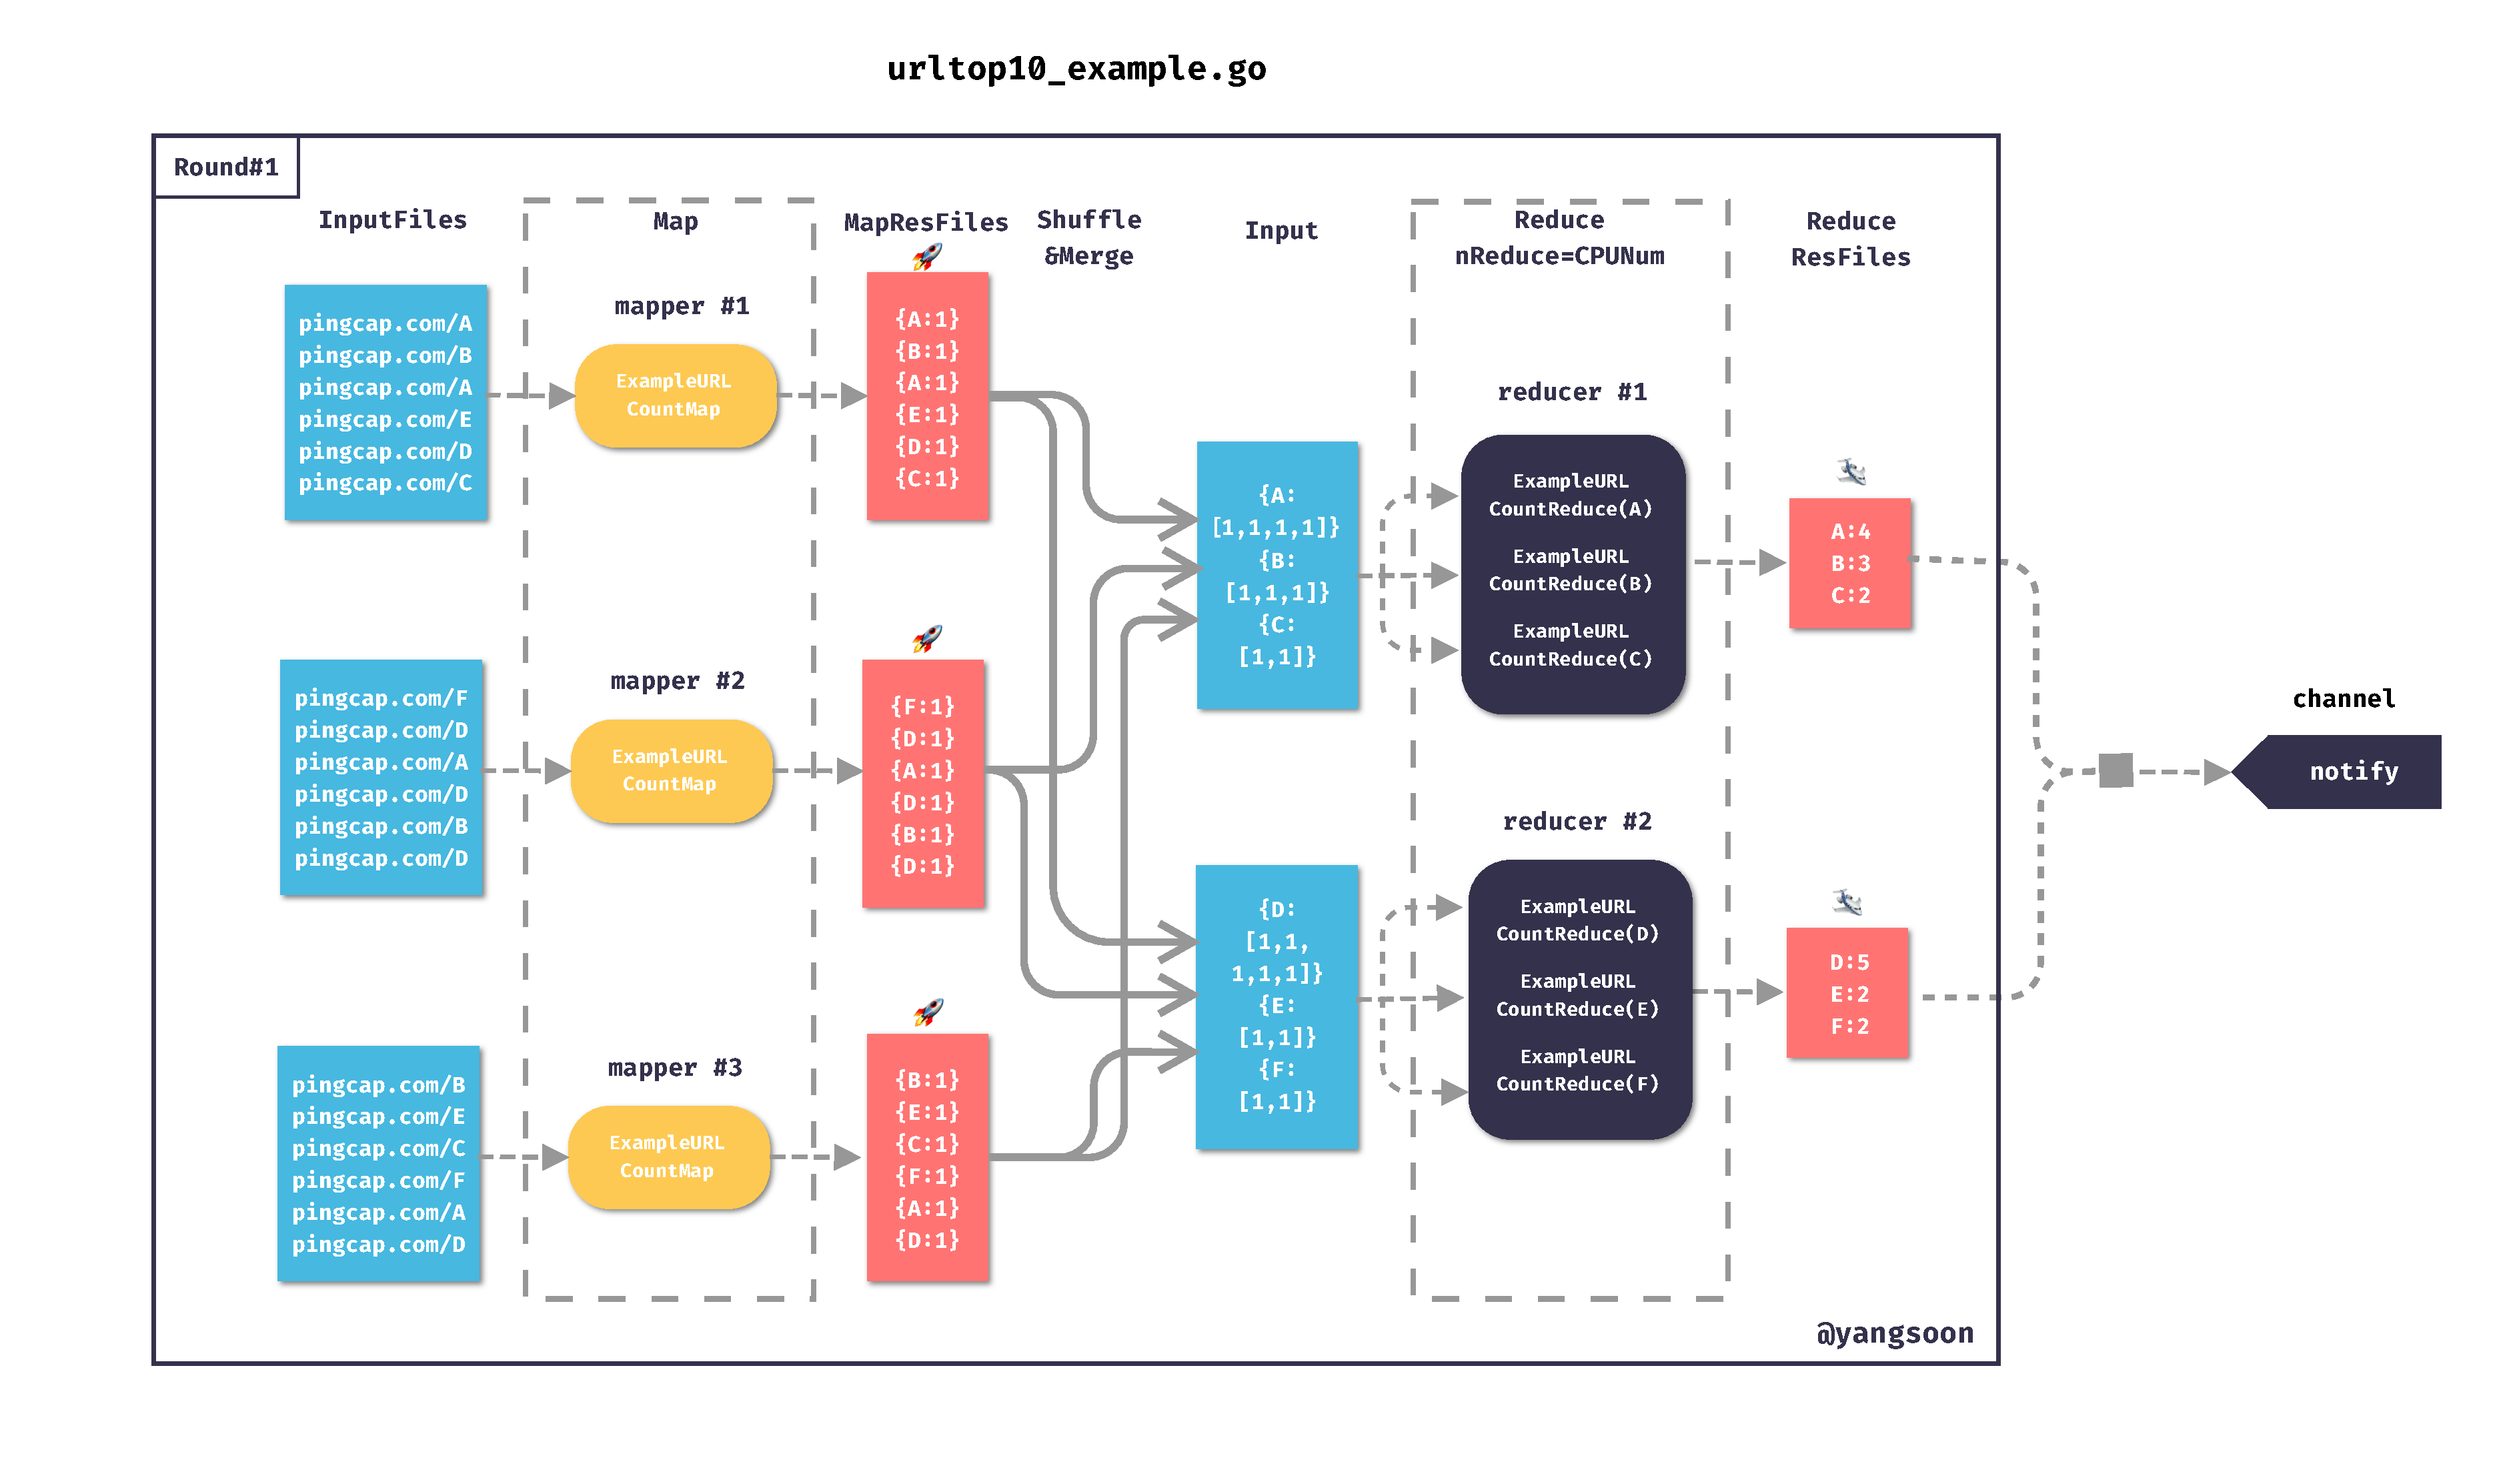
\includegraphics[width=0.9\textwidth]{fig/mr-example-1.pdf}\\
  \caption{urltop10-example-round-1}
  \label{mre1}
\end{figure}
2. 第二轮,map任务从notify管道中读取需要处理的文件,这部分map任务就是简单的将每条数据做一个键值化,
将每条url计数后的结果都分配给唯一的reduce任务,reduce任务只处理一个键值对,
其中value中存储了所有种类url的计算结果,接下来reduce任务计算出topK,
输出到唯一的一个结果文件中。具体的执行过程参考图\ref{mre2}。
\begin{figure}[H]
  \centering
  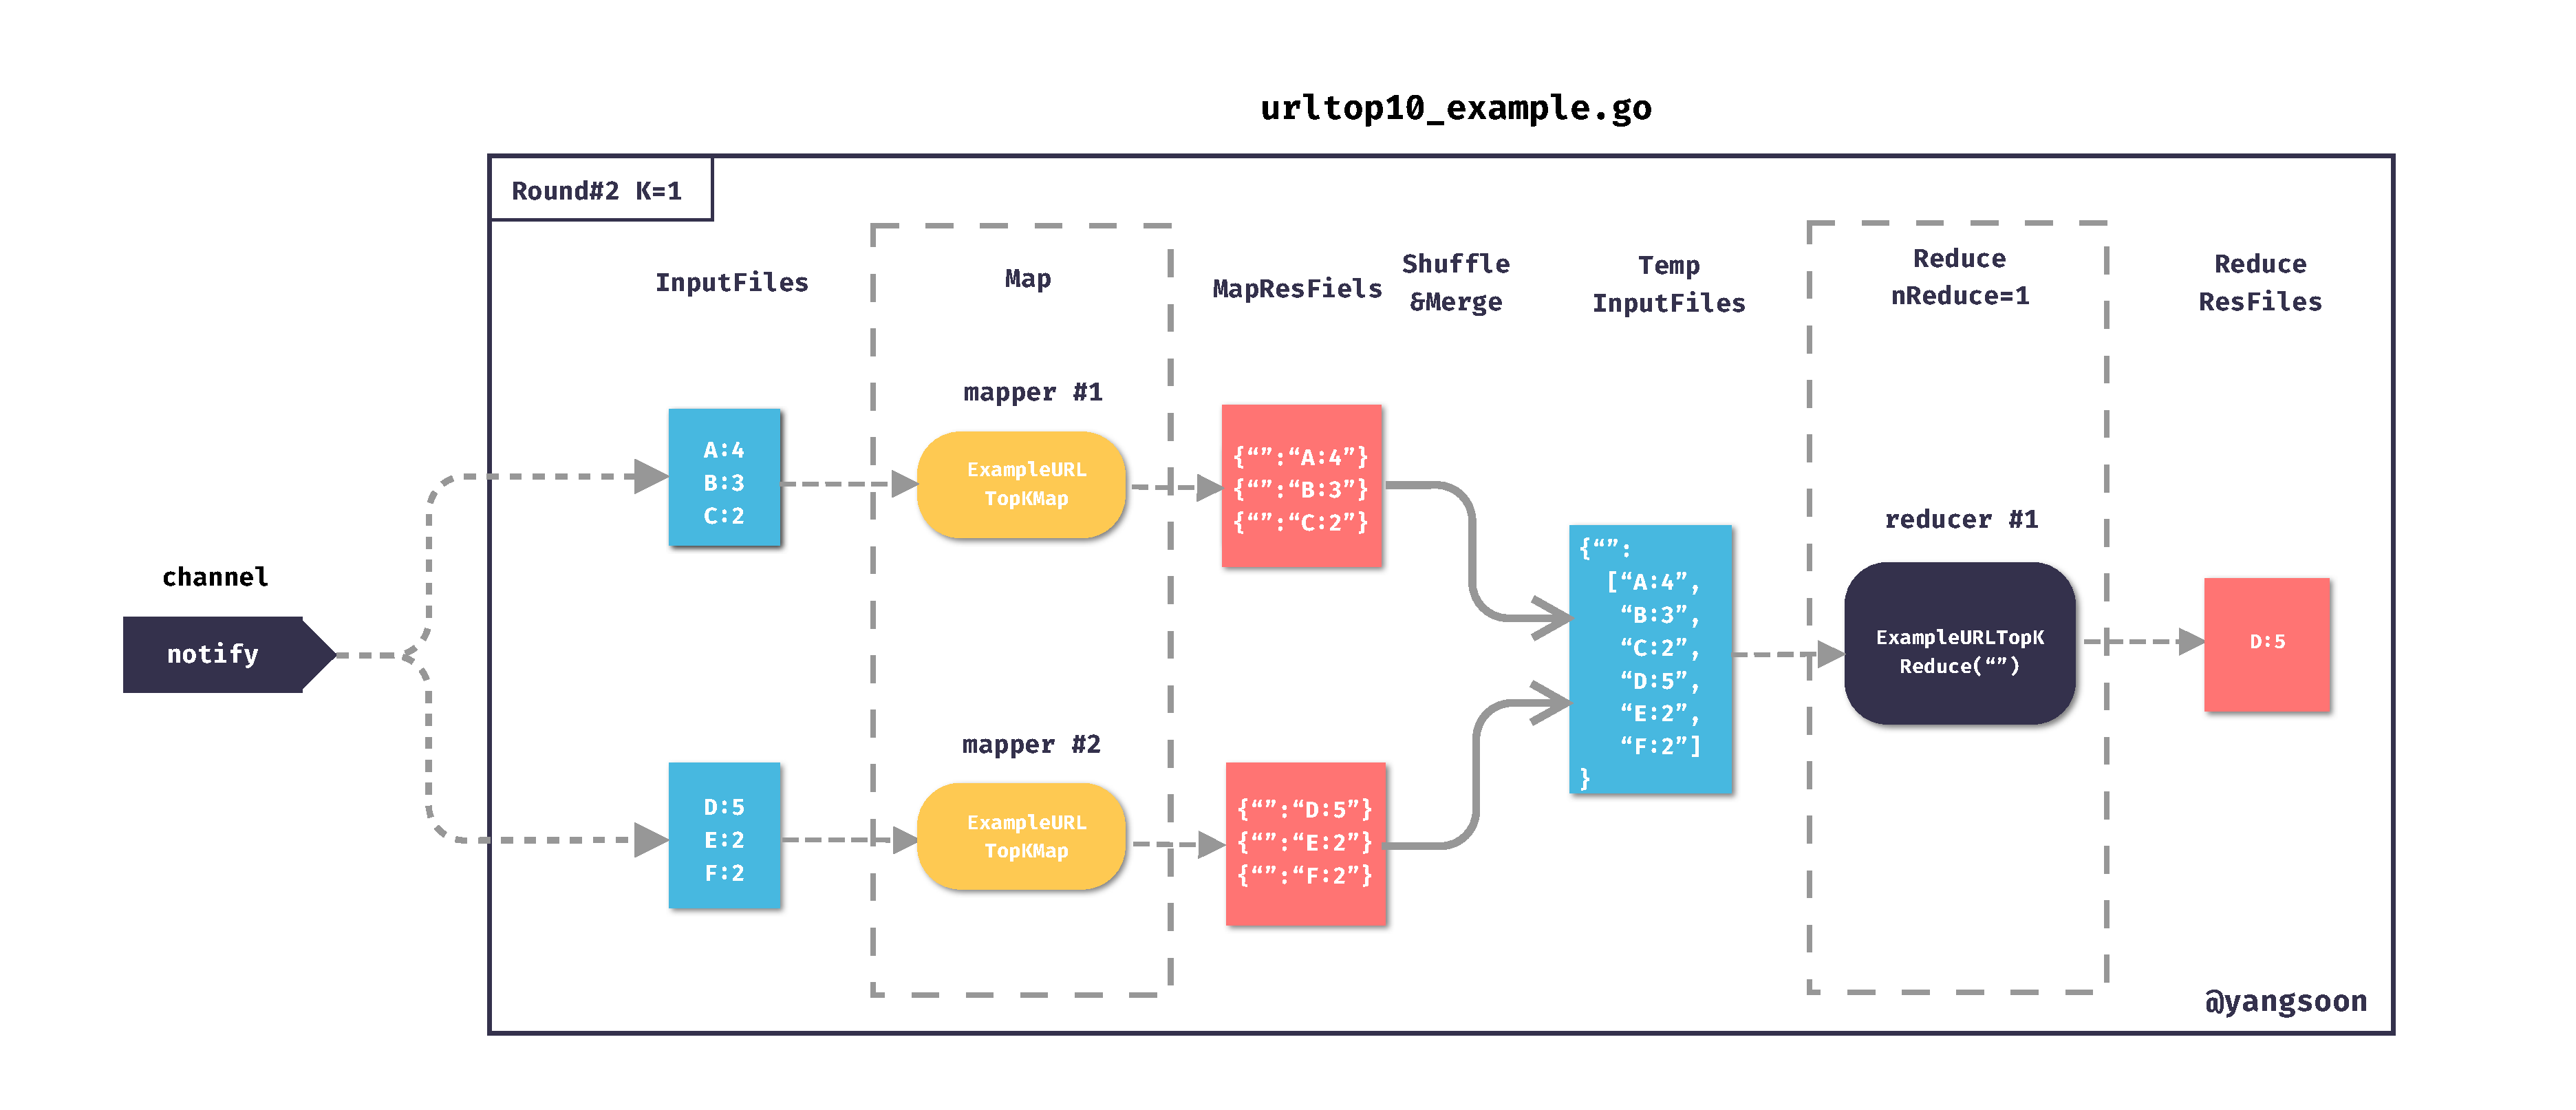
\includegraphics[width=0.7\textwidth]{fig/mr-example-2.pdf}\\
  \caption{urltop10-example-round-2}
  \label{mre2}
\end{figure}

\textbf{第一次优化}

当大概阅读完example的代码之后,我的第一感觉就是example代码有2处可以优化的部分:
\begin{enumerate}
  \item 首先,在第2轮的map任务就可以提前计算每个map中的top10的url,然后将结果发送给reduce任务处理,这样reduce任务的计算压力就会比较小了。
  \item 因为只需要计算出top10即可,不需要对所有的url进行排序,计算top10的算法可以使用堆进行处理,
        维护一个有10个元素的小顶堆,这样也会减少对内存的申请,减少gc时间。
\end{enumerate}

根据这样最初的想法,我实现了第一版的urltop10,和example的代码一样,
也是分成两轮,其中第一轮的代码直接复用example的代码,
第二轮的map任务使用小顶堆来计算top10,然后将结果发送给reduce任务,
reduce任务再对收集来的结果也使用小顶堆来计算top10。

但是,最终的结果不是很理想,多次执行后,时间和example相差无几,时间在630s左右。
下面是对程序的cpu性能分析结果。
\begin{lstlisting}[language=]
  go tool pprof cpu.prof                                                                                                      Time: Oct 4, 2019 at 5:01pm (CST)
  Duration: 10.55mins, Total samples = 24.77mins (234.68%)
  Entering interactive mode (type "help" for commands, "o" for options)
  (pprof) top
  Type: cpu
  Showing nodes accounting for 588.25s, 39.58% of 1486.06s total
  Dropped 377 nodes (cum <= 7.43s)
  Showing top 10 nodes out of 146
        flat  flat%   sum%        cum   cum%
     101.25s  6.81%  6.81%    114.77s  7.72%  encoding/json.stateInString
      76.69s  5.16% 11.97%    164.62s 11.08%  encoding/json.(*decodeState).scanWhile
      66.87s  4.50% 16.47%    189.21s 12.73%  encoding/json.checkValid
      63.91s  4.30% 20.77%     63.91s  4.30%  runtime.pthread_cond_signal
      62.79s  4.23% 25.00%    133.73s  9.00%  runtime.scanobject
      58.89s  3.96% 28.96%     79.60s  5.36%  runtime.findObject
      46.98s  3.16% 32.12%    183.71s 12.36%  runtime.mallocgc
      44.32s  2.98% 35.11%     44.33s  2.98%  encoding/json.unquoteBytes
      33.31s  2.24% 37.35%     94.69s  6.37%  runtime.gcWriteBarrier
      33.24s  2.24% 39.58%     69.77s  4.69%  runtime.mapassign_faststr
\end{lstlisting}

可以看到大部分时间都消耗在了json的解析和gc上,突然我意识到,性能瓶颈不在于排序计算,
而是在于要降低json解析的压力,那么就需要尽量减少中间文件的大小。

\textbf{第二次优化}

继续看example代码,还能发现几个很明显的问题,首先每一轮的map任务都在做一些很简单的事情,
只是对输入结果进行了一下简单的格式化。其次,第一轮的reduce任务每次只能在一组键值对上进行reduce操作,
但是这时候reduce任务上已经有足够的信息来计算局部的topk来对中间结果进行压缩。

根据上面的分析,我进行了第二次的优化,抛弃之前的思路,
具体的执行流程如下图所示, 问题的解决还是通过2轮MapReduce操作进行解决。

第一轮,map任务对输入文件的url进行个数统计,计算每种url的出现次数,
得到一个url和出现次数的结果 然后在对结果格式化的时候进行一个特别的处理,
和之前的处理不同,格式化的key不再是url,而是ihash(url),就是经过hash之后的url值, 
value存储着 url: count形式的字符串,这样处理的原因是这样的话,
map任务中将要发送到同一个reduce work的url都会有相同的key,
这样就能保证每个reduce worker经过shuffle\&merge之后获得的输入信息是只有一个键值对的map对象,
其中包括了所有发送到该work的url统计信息;reduce任务获取到只有一个键值对的map对象后,
首先merge相同url的执行次数,然后计算局部topk,这样输出结果就只包含 K * nReduce 个信息。

\textbf{可以对比下图和上图,在标有小火箭部分的文件,
可以看到第一次中间文件的压缩结果,在标有小飞机部分的中间文件,有更加明显的数据压缩。}
\begin{figure}[H]
  \centering
  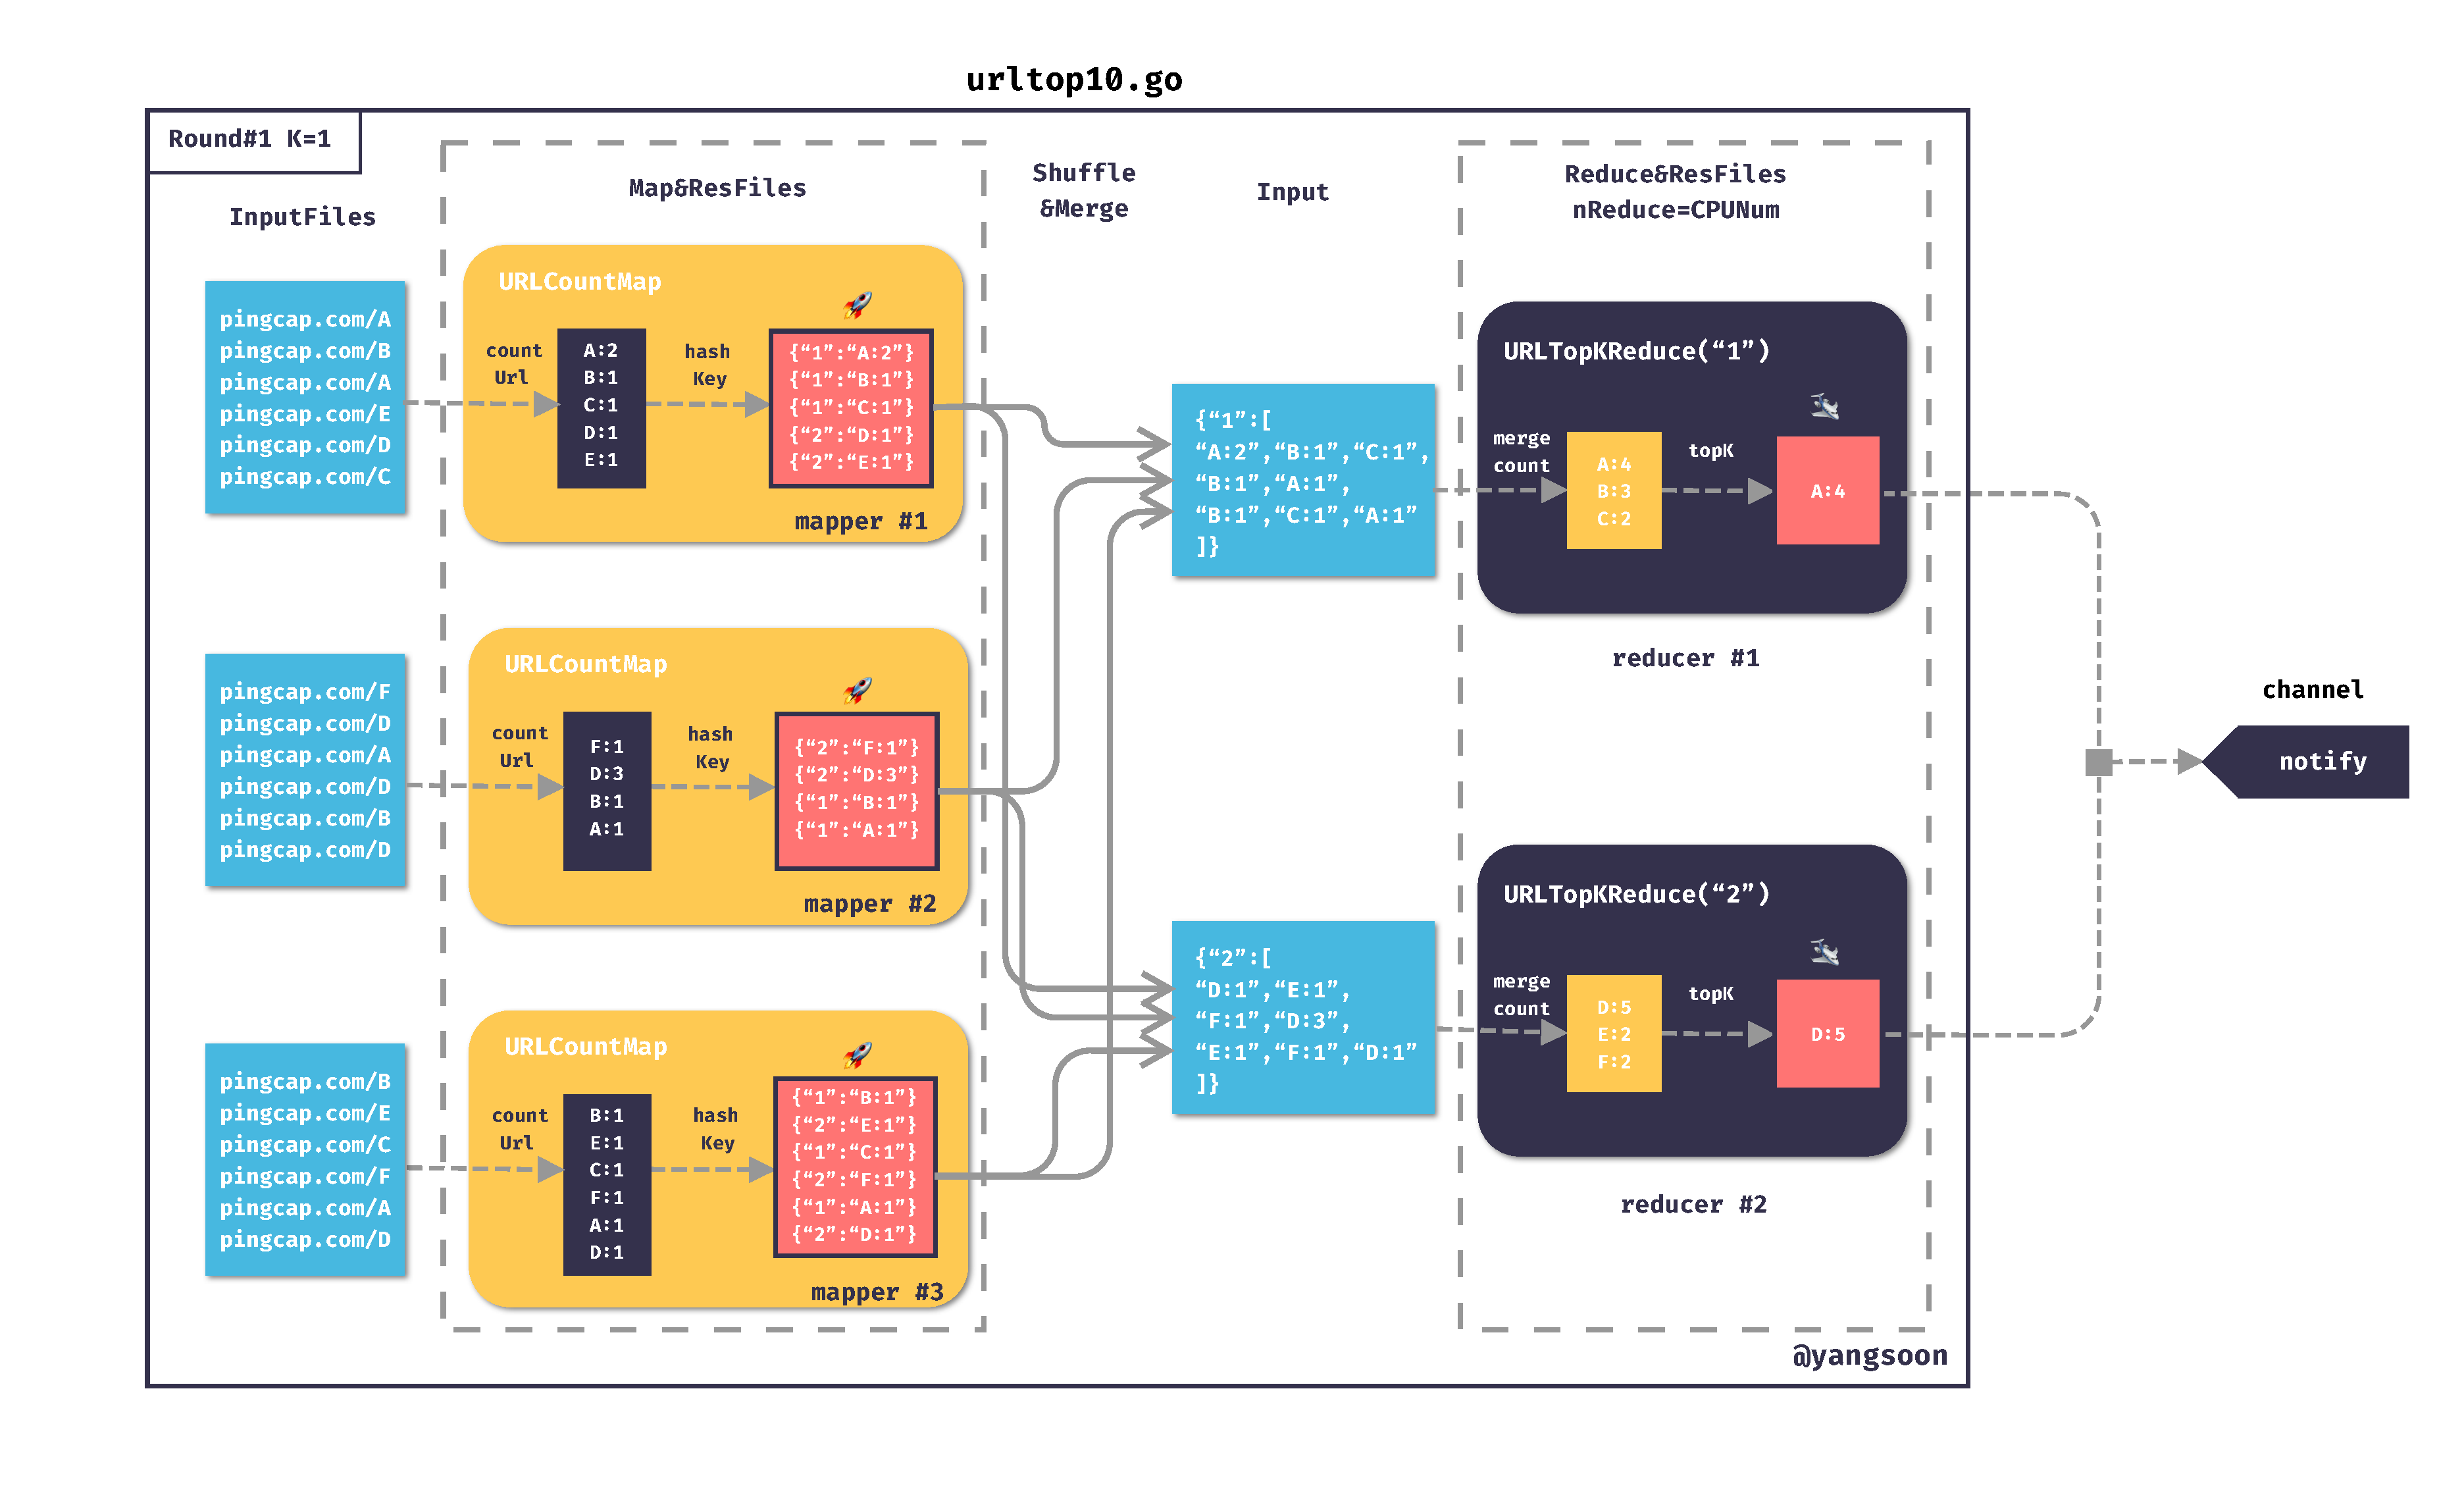
\includegraphics[width=1\textwidth]{fig/mr-1.pdf}\\
  \caption{MapReduce}
  \label{mr1}
\end{figure}
第二轮的操作和example的处理就一样了,这里就不做赘述。
\begin{figure}[H]
  \centering
  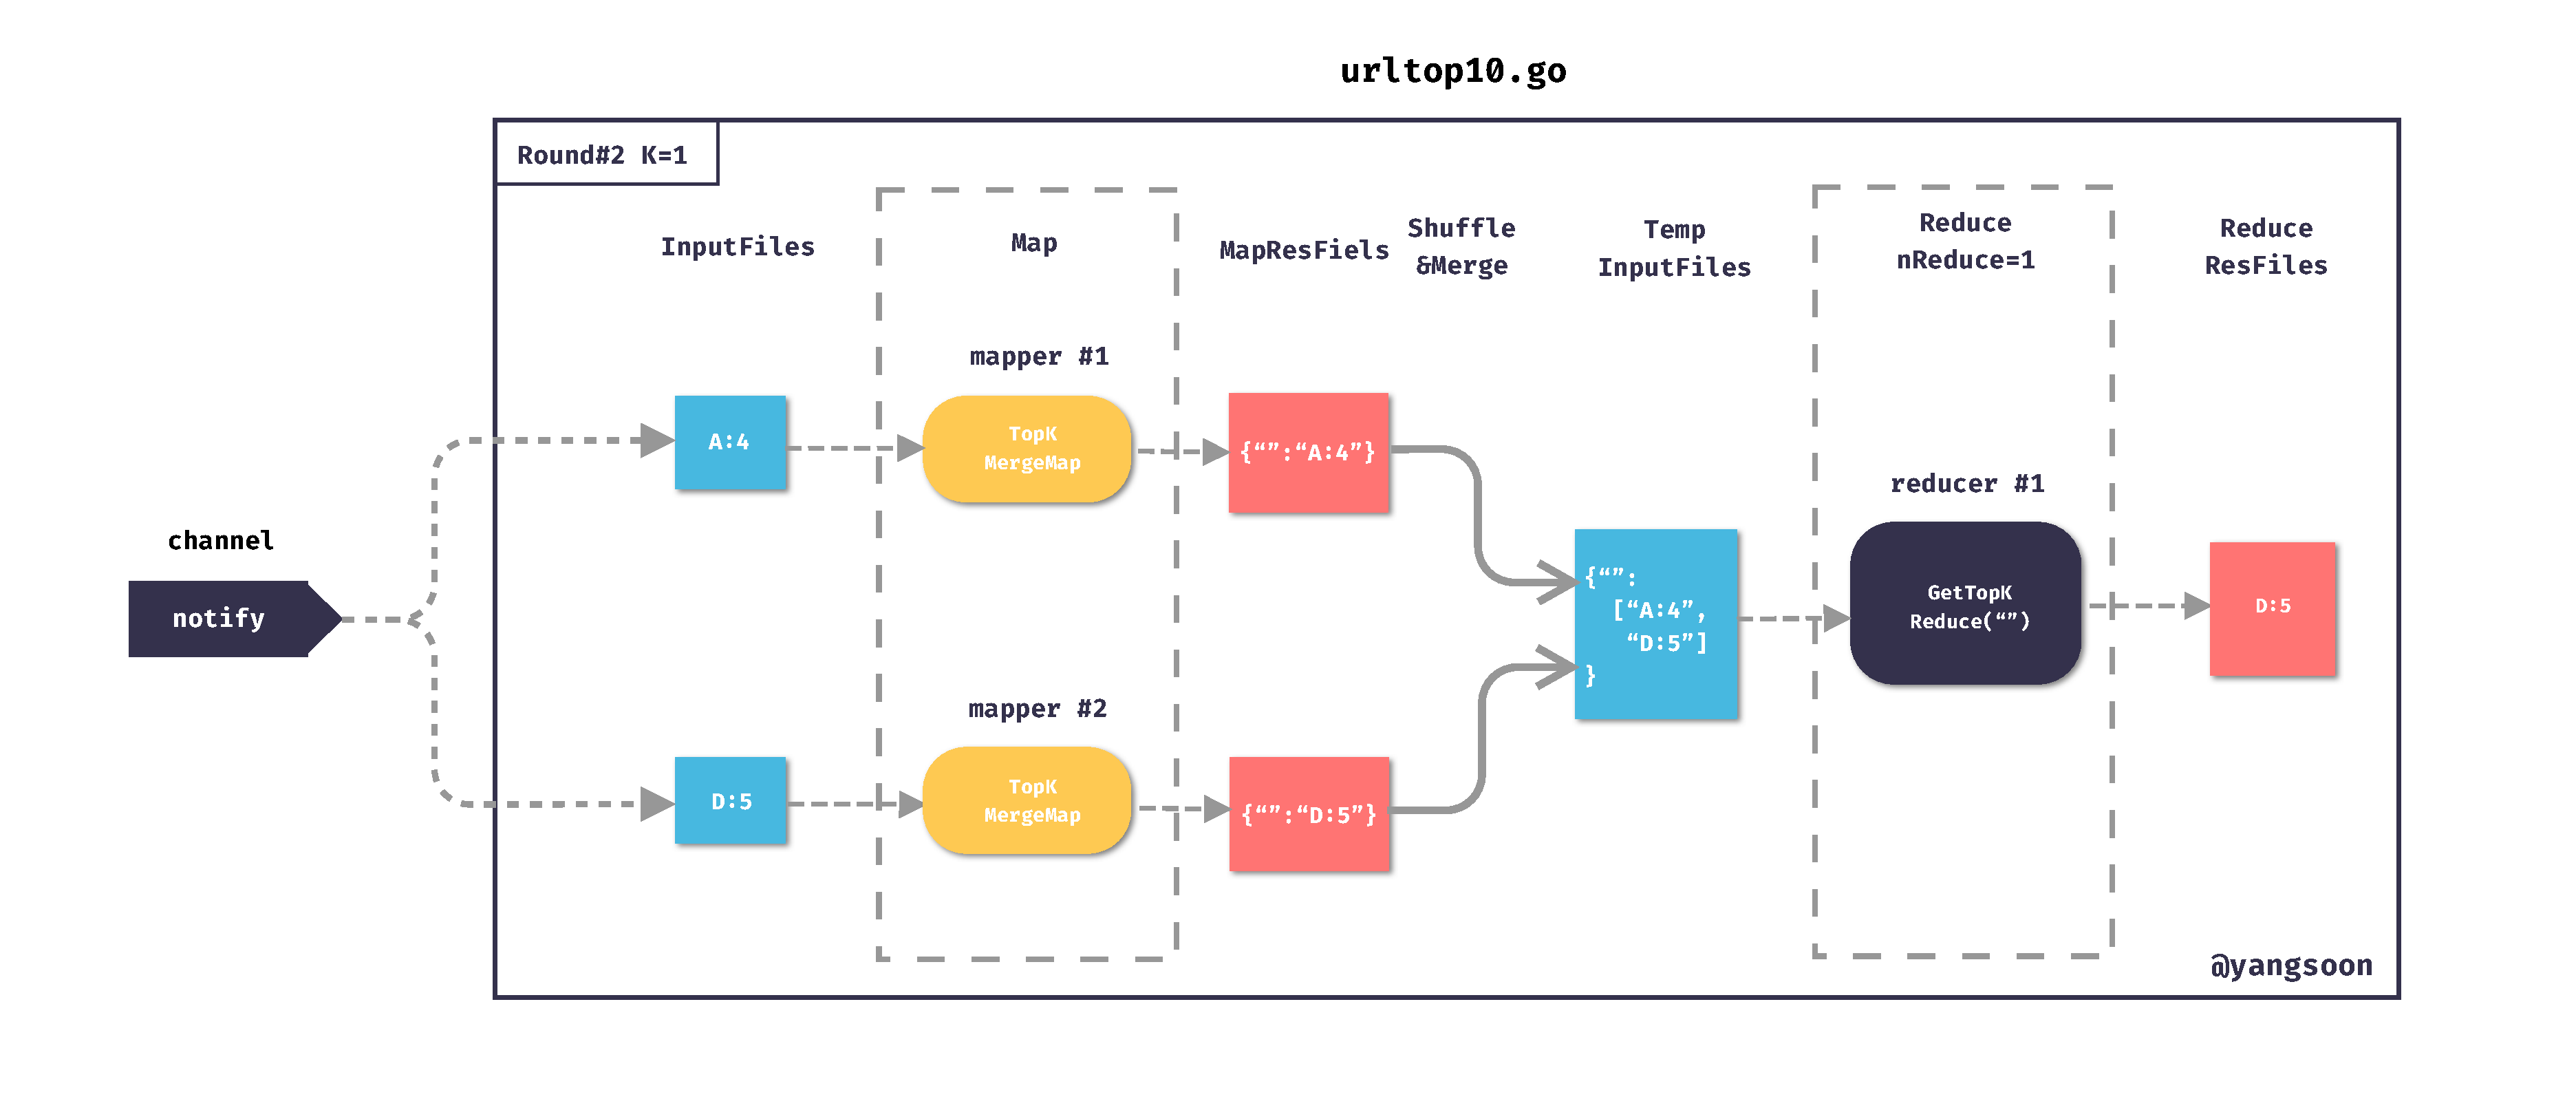
\includegraphics[width=0.8\textwidth]{fig/mr-2.pdf}\\
  \caption{MapReduce}
  \label{sec2:subsec3:fg1}
\end{figure}

之前也考虑过只用一轮MapReduce解决问题,但是思考了一下,发现并不好,
首先map worker的处理逻辑就会比较复杂,而且只能开一个reduce worker 会比较浪费cpu资源。
实际上经过一轮的压缩,第二轮能够较快的执行完。实验显示第二轮的执行时间都在1ms左右。

\textbf{部分代码}
因为主要在first round进行了优化了,所以只列出了round1的相关代码。
\begin{lstlisting}
  func URLTop10(nWorkers int) RoundsArgs {
    var args RoundsArgs
  
    args = append(args, RoundArgs{
      MapFunc:    URLCountMap,
      ReduceFunc: URLCountReduce,
      NReduce:    nWorkers,
    })
  
    args = append(args, RoundArgs{
      MapFunc:    TopKMergeMap,
      ReduceFunc: GetTopKReduce,
      NReduce:    1,
    })
  
    return args
  }
  
  func URLCountMap(filename string, contents string) []KeyValue {
    lines := strings.Split(contents, "\n")
    kv := make(map[string]int, urlKind)
    for _, l := range lines {
      if len(l) == 0 {
        continue
      }
      kv[l] += 1
    }
    kvs := make([]KeyValue, 0, len(lines))
    var buffer bytes.Buffer
    for k, v := range kv {
      buffer.WriteString(k)
      buffer.WriteString(" ")
      buffer.WriteString(strconv.Itoa(v))
  
      kvs = append(kvs, KeyValue{
        Key:   strconv.Itoa(ihash(k) % GetMRCluster().NWorkers()),
        Value: buffer.String(),
      })
  
      buffer.Reset()
    }
    return kvs
  }
  
  func URLCountReduce(key string, values []string) string {
  
    kv := make(map[string]int, urlKind)
  
    for _, value := range values {
      if len(value) == 0 {
        continue
      }
      tmp := strings.Split(value, " ")
      n, err := strconv.Atoi(tmp[1])
      if err != nil {
        panic(err)
      }
      kv[tmp[0]] += n
    }
  
    topk := Top10(kv)
  
    buf := new(bytes.Buffer)
    for i := 0; i < len(topk); i++ {
      fmt.Fprintf(buf, "%s %d\n", topk[i].url, topk[i].cnt)
    }
    return buf.String()
  }  
\end{lstlisting}

\textbf{其他优化}
urlcountmap urlcountreduce 申请空间过大
// 后续补充
\end{document}

